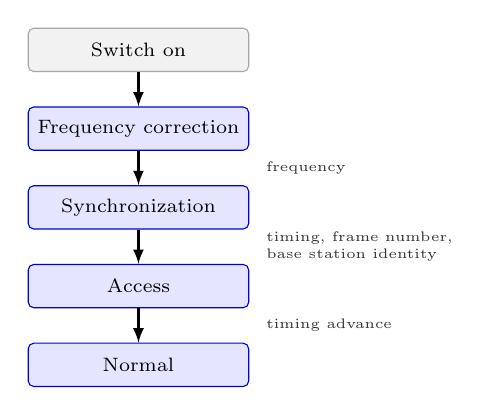
\begin{tikzpicture}[
    >=latex,
    stage/.style={draw=blue!85!black, fill=blue!10, rounded corners=2pt, minimum width=2.8cm, minimum height=0.55cm, font=\scriptsize, align=center},
    learned/.style={anchor=west, font=\tiny, align=left, text=gray!40!black}
]
    % Burst sequence of a terminal after switch-on
    \node[stage, fill=gray!10, draw=gray!70] (on) at (0,0) {Switch on};
    \node[stage] (fb) at (0,-1.0) {Frequency correction};
    \node[stage] (sb) at (0,-2.0) {Synchronization};
    \node[stage] (ab) at (0,-3.0) {Access};
    \node[stage] (nb) at (0,-4.0) {Normal};

    \draw[->, thick] (on) -- (fb);
    \draw[->, thick] (fb) -- (sb);
    \draw[->, thick] (sb) -- (ab);
    \draw[->, thick] (ab) -- (nb);

    % What the terminal knows after each step
    \node[learned] at (1.5,-1.5) {frequency};
    \node[learned] at (1.5,-2.5) {timing, frame number,\\base station identity};
    \node[learned] at (1.5,-3.5) {timing advance};
\end{tikzpicture}
